% Mayer-Vietoris on the sphere: two overlapping caps and the band. Generated by a short script.
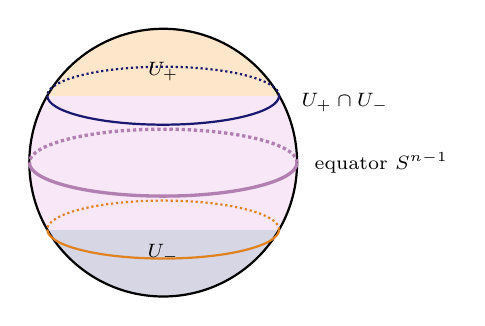
\begin{tikzpicture}[font=\scriptsize]
\begin{scope}\clip (0,0) circle (1.7);
\fill[BurntOrange!18] (-1.7,-0.85) rectangle (1.7,1.7);
\fill[MidnightBlue!18] (-1.7,0.85) rectangle (1.7,-1.7);
\fill[Plum!25] (-1.7,-0.85) rectangle (1.7,0.85);
\end{scope}
\draw[thick] (0,0) circle (1.7);
\draw[BurntOrange!90!black,thick] (-1.472,-0.850) arc[start angle=180,end angle=360,x radius=1.472,y radius=0.368];
\draw[BurntOrange!90!black,thick,densely dotted] (1.472,-0.850) arc[start angle=0,end angle=180,x radius=1.472,y radius=0.368];
\draw[MidnightBlue,thick] (-1.472,0.850) arc[start angle=180,end angle=360,x radius=1.472,y radius=0.368];
\draw[MidnightBlue,thick,densely dotted] (1.472,0.850) arc[start angle=0,end angle=180,x radius=1.472,y radius=0.368];
\draw[Plum!80!black,very thick] (-1.7,0) arc[start angle=180,end angle=360,x radius=1.7,y radius=0.425];
\draw[Plum!80!black,very thick,densely dotted] (1.7,0) arc[start angle=0,end angle=180,x radius=1.7,y radius=0.425];
\node at (0,1.1560000000000001) {$U_+$};
\node at (0,-1.1560000000000001) {$U_-$};
\node[right] at (1.8,0) {equator $S^{n-1}$};
\node[right] at (1.6300000000000001,0.765) {$U_+\cap U_-$};
\end{tikzpicture}
